%definira klasu dokumenta 
\documentclass[12pt]{report} 

%prostor izmedu naredbi \documentclass i \begin{document} se zove uvod. U njemu se nalaze naredbe koje se odnose na cijeli dokument

%osnovni LaTex ne može riješiti sve probleme, pa se koriste različiti paketi koji olakšavaju izradu željenog dokumenta
\usepackage[croatian]{babel} 
\usepackage{amssymb}
\usepackage{amsmath}
\usepackage{txfonts}
\usepackage{mathdots}
\usepackage{titlesec}
\usepackage{array}
\usepackage{lastpage}
\usepackage{etoolbox}
\usepackage{tabularray}
\usepackage{color, colortbl}
\usepackage{adjustbox}
\usepackage{geometry}
\usepackage[classicReIm]{kpfonts}
\usepackage{hyperref}
\usepackage{fancyhdr}
\usepackage{listings}
\usepackage{float}
\usepackage{setspace}

\restylefloat{table}


\patchcmd{\chapter}{\thispagestyle{plain}}{\thispagestyle{fancy}}{}{} %redefiniranje stila stranice u paketu fancyhdr

%oblik naslova poglavlja
\titleformat{\chapter}{\normalfont\huge\bfseries}{\thechapter.}{20pt}{\Huge}
\titlespacing{\chapter}{0pt}{0pt}{40pt}


\linespread{1.3} %razmak između redaka

\geometry{a4paper, left=1in, top=1in,}  %oblik stranice

\hypersetup{ colorlinks, citecolor=black, filecolor=black, linkcolor=black,	urlcolor=black }   %izgled poveznice


%prored smanjen između redaka u nabrajanjima i popisima
\newenvironment{packed_enum}{
	\begin{enumerate}
		\setlength{\itemsep}{0pt}
		\setlength{\parskip}{0pt}
		\setlength{\parsep}{0pt}
	}{\end{enumerate}}

\newenvironment{packed_item}{
	\begin{itemize}
		\setlength{\itemsep}{0pt}
		\setlength{\parskip}{0pt}
		\setlength{\parsep}{0pt}
	}{\end{itemize}}




%boja za privatni i udaljeni kljuc u tablicama
\definecolor{LightBlue}{rgb}{0.9,0.9,1}
\definecolor{LightGreen}{rgb}{0.9,1,0.9}

%Promjena teksta za dugačke tablice
\DefTblrTemplate{contfoot-text}{normal}{Nastavljeno na idućoj stranici}
\SetTblrTemplate{contfoot-text}{normal}
\DefTblrTemplate{conthead-text}{normal}{(Nastavljeno)}
\SetTblrTemplate{conthead-text}{normal}
\DefTblrTemplate{middlehead,lasthead}{normal}{Nastavljeno od prethodne stranice}
\SetTblrTemplate{middlehead,lasthead}{normal}

%podesavanje zaglavlja i podnožja

\pagestyle{fancy}
\lhead{Programsko inženjerstvo}
\rhead{FlipMemo}
\lfoot{Olimplusplus}
\cfoot{stranica \thepage/\pageref{LastPage}}
\rfoot{\today}
\renewcommand{\headrulewidth}{0.2pt}
\renewcommand{\footrulewidth}{0.2pt}


\begin{document} 
	
	
	
	\begin{titlepage}
		\begin{center}
			\vspace*{\stretch{1.0}} %u kombinaciji s ostalim \vspace naredbama definira razmak između redaka teksta
			\LARGE Programsko inženjerstvo\\
			\large Ak. god. 2023./2024.\\
			
			\vspace*{\stretch{3.0}}
			
			\huge FlipMemo\\
			\Large Dokumentacija, Rev. \textit{2}\\
			
			\vspace*{\stretch{12.0}}
			\normalsize
			Grupa: \textit{Olimplusplus}\\
			Voditelj: \textit{Duje Štolfa}\\
			
			
			\vspace*{\stretch{1.0}}
			Datum predaje: \textit{19. 1. 2024.}\\
	
			\vspace*{\stretch{4.0}}
			
			Nastavnik: \textit{Goran Rajić}\\
		
		\end{center}

	
	\end{titlepage}

	
	\tableofcontents


	\chapter{Dnevnik promjena dokumentacije}
		
		\textbf{\textit{Kontinuirano osvježavanje}}\\
				
		
		\begin{longtblr}[
				label=none
			]{
				width = \textwidth, 
				colspec={|X[2]|X[11]|X[5]|X[4]|}, 
				rowhead = 1
			}
			\hline
			\textbf{Rev.}	& \textbf{Opis promjene/dodatka} & \textbf{Autori} & \textbf{Datum}\\[3pt] \hline
			0.1 & Napravljen predložak.	& Duje Štolfa & 25.10.2023. 		\\[3pt] \hline 
			0.2	& Opis projektnog zadatka. & Gabrijel Čobanov \newline Karlo Kuzle & 28.10.2023. 	\\[3pt] \hline 
			0.3 & Razrađeni funkcionalni zahtjevi, \newline aktori i dionici. \newline Nabrojani \textit{Use Caseovi}. & Nina Bulić \newline Duje Štolfa & 29.10.2023. \\[3pt] \hline 
			0.4 & Opisani obrasci uporabe \newline i ostali zahtjevi. & Frane Kuzmanić \newline Gabijel Čobanov \newline Nikša Brala \newline Karlo Kuzle \newline Nina Bulić \newline Duje Štolfa \newline Ivo Žilić & 31.10.2023.\\[3pt] \hline 
			0.7 & Dijagrami obrazaca uporabe & Frane Kuzmanić & 31.11.2023. \\[3pt] \hline 
			0.6 & Dodani sekvencijski dijagrami \newline i njihovi opisi &  Nina Bulić \newline Duje Štolfa \newline Ivo Žilić & 2.11.2023. \\[3pt] \hline 
			0.7 & Dijagram baze podataka & Nikša Brala & 5.11.2023. \\[3pt] \hline
			0.8 & Opis baze i tablica baze podataka & Karlo Kuzle & 7.11.2023. \\[3pt] \hline 
			0.9 & Dodan opis arhitekture sustava & Duje Štolfa \newline Gabrijel Čobanov \newline Frane Kuzmanić & 10.11.2023. \\[3pt] \hline 
			0.10 & Dijagrami razreda & Nikša Brala & 11.11.2023. \\[3pt] \hline 
			0.11 & Opis dijagrama razreda & Gabrijel Čobanov \newline Nina Bulić \newline Ivo Žilić \newline Duje Štolfa & 13.11.2023. \\[3pt] \hline 
			\textbf{1.0} & Prva revizija dokumentacije & * & 17.11.2023. \\[3pt] \hline 
		\end{longtblr}
	
	
		\textit{Moraju postojati glavne revizije dokumenata 1.0 i 2.0 na kraju prvog i drugog ciklusa. Između tih revizija mogu postojati manje revizije već prema tome kako se dokument bude nadopunjavao. Očekuje se da nakon svake značajnije promjene (dodatka, izmjene, uklanjanja dijelova teksta i popratnih grafičkih sadržaja) dokumenta se to zabilježi kao revizija. Npr., revizije unutar prvog ciklusa će imati oznake 0.1, 0.2, …, 0.9, 0.10, 0.11.. sve do konačne revizije prvog ciklusa 1.0. U drugom ciklusu se nastavlja s revizijama 1.1, 1.2, itd.}
	\chapter{Opis projektnog zadatka}
	
Cilj ovog projekta je razvoj aplikacije FlipMemo u svrhu učenja riječi na stranom jeziku. FlipMemo je namijenjen svima koji žele unaprijediti svoje znanje na interaktivan i efikasan način. Aplikacija omogućuje početnicima kao i naprednim korisnicima razvijanje svoje vještine razumijevanja, čitanja i pisanja stranog jezika. Učenje se oslanja na tehniku ponavljanja s rastućim vremenskim razmacima. Aplikaciju će moći koristiti bilo tko zainteresiran za učenje jezika, te sve što je potrebno je adresa elektroničke pošte.

\section{Ponavljanje s rastućim vremenskim razmakom}

SR (iz engleskog „spaced repetition”) tehnika je napravljena tako da iskoristi psihološki efekt prisjećanja. Naime, ljudi prirodno zaboravljaju informacije koje ne koriste često, jer ljudska memorija nije beskonačna, pa stvari koje nisu dio svakodnevice postaju dio zaborava. Ta činjenica još više vrijedi za nove informacije. Informacija koju ne koristimo ili ne vežemo s iskustvom se jednostavno ne smatra važnom, stoga se lako zaboravi. SR tehnika rješava ovaj problem tako što informacije koje želimo naučiti (u našem slučaju riječi jezika) pretvara u dio svakodnevice.

\begin{figure}[H]
	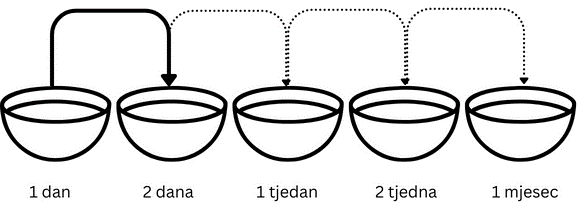
\includegraphics[scale=0.8]{slike/spaced_repetition.png} 
	\centering
	\caption{Ilustracija sustava za učenje s pet posuda}
	\label{fig:spacedrepetition}
\end{figure}

Kako bismo lakše razumjeli ovaj način učenja, zamislimo nekoliko posuda, kao na slici \ref{fig:spacedrepetition}. U svakoj posudi se nalaze kartice s informacijama koje korisnik želi naučiti. Na karticama se nalazi pitanje i odgovor. Svaka posuda je označena sa svojim vremenskim intervalom. Svaka kartica na koju se da točan odgovor ide u sljedeću posudu. Svaka kartica na koju se da netočan odgovor, ide u prvu posudu. Ako se na karticu odgovori točno, a bila je izvađena iz zadnje posude, kartica izlazi iz sistema i ta informacija se smatra naučenom. Korisnik na početku sesije učenja vadi sve kartice iz prve posude, te odgovara na pitanja. One na koje odgovori točno, stavlja u posudu od dva dana, one na koje odgovori netočno, ostavlja u posudu od jednog dana. Kad završi sa svim pitanjima, sesija je za taj dan gotova. Ako korisnik odluči učiti odmah dan nakon, može vaditi kartice iz prve posude, ali ne iz druge. Tek nakon prolaska dva dana može opet uzeti kartice iz druge posude.

Cilj je u tome da se informacije koje teže ili manje pamte, viđaju češće. Stvari koje korisnik zna ili razumije lakše, viđa manje, čime se može fokusirati na nedostatke u svom znanju.

\eject
\section{Opis aplikacije}

Aplikacija je kolekcija rječnika iz kojih se mogu učiti riječi odabranog jezika. Rječnik je kolekcija međusobno značenjem povezanih riječi. Svaka riječ ima svoj prijevod na hrvatski, te prijevode na implementirane strane jezike, značenje tih riječi, pomoćne rečenice unutar kojih se ta riječ koristi i audiozapis izgovora riječi na svakom od njih. Riječi dodaju administratori riječi, čije ovlasti može dati jedan korijenski administrator. Korisnici imaju pristup svim rječnicima odabranog jezika za učenje, te četiri načina učenja.

Riječi i rječnici su odgovornost administratora riječi. Pri dodavanju riječi u sustav, administrator je dužan pobrinuti se za točnost prijevoda i značenja, kao i pomoćne rečenice i audiozapisa izgovora riječi. U tom poslu mu pomaže API. Jednu riječ može dijeliti više rječnika. 

\subsection{Načini učenja} 

U aplikaciji su predviđena četiri načina učenja, kako bi savladavanje gradiva išlo što lakše i brže:
\begin{description}
	\item[Foreign promt --- native translation:] Korisniku je prikazana riječ stranog jezika. Ponuđeno mu je nekoliko riječi na hrvatskom jeziku od kojih on mora odabrati onu koja je najbolji prijevod strane riječi. Riječi koje se nude kao odgovori biraju se iz trenutno aktivnog rječnika, tj. rječnika iz kojeg se uči. 
	\item[Native translation --- foreign promt:] Korisniku je prikazana riječ na hrvatskom jeziku, te mu je ponuđeno nekoliko riječi na stranom jeziku. Korisnik od njih mora odabrati onu koja je točan prijevod riječi na hrvatskom jeziku.
	\item[Listen and translate:] Korisnik sluša audiozapis izgovora trenutne riječi na odabranom jeziku učenja. Korisnik treba napisati riječ koju je čuo. Time se provjerava razumije li korisnik razlike u izgovoru riječi kao i njihovo pisanje.
	\item[Record your translation:] Korisnik dobiva riječ na jeziku koji uči i opciju za snimanje glasa. Potrebno je točno izgovoriti riječ prikazanu na ekranu. Ocjena izgovora može biti brojka od jedan do deset, čime korisnik dobiva povratnu informaciju o svom izgovoru.
\end{description}

Nakon svakog odgovorenog pitanja, korisnik dobiva povratnu informaciju o točnosti odgovora. Kad korisnik završi sa sesijom učenja i prođe sve riječi za taj dan aplikacija mu javlja da je za taj dan s tim rječnikom gotov. 

\eject

	\chapter{Specifikacija programske potpore}
		
	\section{Funkcionalni zahtjevi}
			
			\textbf{\textit{dio 1. revizije}}\\
			
			\textit{Navesti \textbf{dionike} koji imaju \textbf{interes u ovom sustavu} ili  \textbf{su nositelji odgovornosti}. To su prije svega korisnici, ali i administratori sustava, naručitelji, razvojni tim.}\\
				
			\textit{Navesti \textbf{aktore} koji izravno \textbf{koriste} ili \textbf{komuniciraju sa sustavom}. Oni mogu imati inicijatorsku ulogu, tj. započinju određene procese u sustavu ili samo sudioničku ulogu, tj. obavljaju određeni posao. Za svakog aktora navesti funkcionalne zahtjeve koji se na njega odnose.}\\
			
			
			\noindent \textbf{Dionici:}
			
			\begin{packed_enum}
				
				\item Dionik 1
				\item Dionik 2				
				\item ...
				
			\end{packed_enum}
			
			\noindent \textbf{Aktori i njihovi funkcionalni zahtjevi:}
			
			
			\begin{packed_enum}
				\item  \underbar{Aktor 1 (inicijator) može:}
				
				\begin{packed_enum}
					
					\item funkcionalnost 1
					\item funkcionalnost 2
					\begin{packed_enum}
						
						\item  podfunkcionalnost 1 
						\item  podfunkcionalnost 2
				
					\end{packed_enum}
					\item  funkcionalnost 3
					
				\end{packed_enum}
			
				\item  \underbar{Aktor 2 (sudionik) može:}
				
				\begin{packed_enum}
					
					\item funkcionalnost 1
					\item funkcionalnost 2
					
				\end{packed_enum}
			\end{packed_enum}
			
			\eject 


\subsection{Obrasci uporabe}

\subsubsection{Opis obrazaca uporabe}

\noindent \underbar{\textbf{UC$<$broj obrasca$>$ - Prijava u sustav}}
\begin{packed_item}

	\item \textbf{Glavni sudionik: } Učenik ili administrator
	\item \textbf{Cilj: } Dobivanje pristupa učeničkom ili administratorskom sučelju
	\item \textbf{Sudionici: } Baza podataka
	\item \textbf{Preduvjet: } -
	\item  \textbf{Opis osnovnog tijeka:}
	
	\item[] \begin{packed_enum}

		\item Korisnik aplikacije unosi svoj e-mail i lozinku
		\item Sustav provjerava postoji li račun s istim podacima
		\item Ako su podaci ispravni, sustav preusmjerava korisnika na zaslon za odabir jezika (nastavak UC Pregledavanje i odabir jezika)

	\end{packed_enum}
	
	\item  \textbf{Opis mogućih odstupanja:}
	
	\item[] \begin{packed_item}

		\item[2.a] Neispravan e-mail ili lozinka
		\item[] \begin{packed_enum}
			
			\item Sustav obavještava korisnika o grešci
			
		\end{packed_enum}
		
	\end{packed_item}
\end{packed_item}


\noindent \underbar{\textbf{UC$<$broj obrasca$>$ - Pregledavanje i odabir jezika}}
\begin{packed_item}

	\item \textbf{Glavni sudionik: } Učenik ili administrator riječi
	\item \textbf{Cilj: } Odabrati željeni jezik iz popisa dostupnih jezika
	\item \textbf{Sudionici: } Baza podataka
	\item \textbf{Preduvjet: } UC Prijava u sustav
	\item  \textbf{Opis osnovnog tijeka:}
	
	\item[] \begin{packed_enum}

		\item Sustav korisniku prikazuje popis dostupnih jezika
		\item Korisnik odabire jezik
		\item Sustav preusmjerava:
		
		\item[] \begin{packed_item}

			\item učenika na zaslon za odabir rječnika (UC Pregledavanje i odabir rječnika)
			\item administratora na zaslon za upravljanje riječima i rječnicima
		
		\end{packed_item}

	\end{packed_enum}
	
\end{packed_item}

\noindent \underbar{\textbf{UC$<$broj obrasca$>$ - Potvrda brisanja elementa}}
\begin{packed_item}

	\item \textbf{Glavni sudionik: } Učenik ili administrator
	\item \textbf{Cilj: } Upozoriti korisnika i potvrditi brisanje bilo kojeg elementa sustava
	\item \textbf{Sudionici: } Baza podataka
	\item \textbf{Preduvjet: } Pohranjen je identifikator elementa kojeg želimo izbrisati	
	\item  \textbf{Opis osnovnog tijeka:}
	
	\item[] \begin{packed_enum}

		\item Sustav korisniku prikazuje popis dostupnih jezika
		\item Korisnik odabire jezik
		\item Sustav preusmjerava:
		
		\item[] \begin{packed_item}

			\item Korisniku je prikazan dijaloški okvir s porukom upozorenja o posljedicama brisanja te gumbovima "Obriši" i "Odustani"
			\item Korisnik potvrđuje brisanje klikom na gumb "Obriši"
			\item Odabrani element briše se iz baze podataka
		
		\end{packed_item}

	\end{packed_enum}

	\item  \textbf{Opis mogućih odstupanja:}
	
	\item[] \begin{packed_item}

		\item[2.a] Korisnik odustaje od brisanja
		\item[] \begin{packed_enum}
			
			\item Odabrani element ne briše se iz baze podataka
			
		\end{packed_enum}
		
	\end{packed_item}
	
\end{packed_item}

\noindent \underbar{\textbf{UC$<$broj obrasca$>$ - Stvaranje riječi}}
\begin{packed_item}

	\item \textbf{Glavni sudionik: } Admin riječi (nadalje Radmin)
	\item \textbf{Cilj: } Mogućnost pregledavanja svih riječi za zadani jezik
	\item \textbf{Sudionici: } Baza podataka
	\item \textbf{Preduvjet: } Prijavljivanje u Radmin račun, odabran jezik, Radmin se nalazi na stranici za pregled riječi (UC stvaranje riječi)	
	\item  \textbf{Opis osnovnog tijeka:}
	
	\item[] \begin{packed_enum}
		
		\item Radmin odabire opciju dodavanja riječi u sustav
		\item Dobiva ekran na kojem se nalaze prostori za unos teksta
		\item Radmin unosi riječ, pri čemu pomaže API
		\item Radmin unosi prijevod riječi, pri čemu pomaže API
		\item Radmin unosi značenje riječi koju dobiva iz API-ja
		\item Radmin unosi pomoćnu frazu koju dobiva iz API-ja
		\item Radmin unosi zvučnu datoteku izgovora riječi na odabranom jeziku

	\end{packed_enum}
	
\end{packed_item}


\noindent \underbar{\textbf{UC$<$broj obrasca$>$ - Uređivanje riječi}}
\begin{packed_item}

	\item \textbf{Glavni sudionik: } Admin riječi (nadalje Radmin)
	\item \textbf{Cilj: } Mogućnost pregledavanja svih riječi za zadani jezik
	\item \textbf{Sudionici: } Baza podataka
	\item \textbf{Preduvjet: } Prijavljivanje u Radmin račun, postojanje riječi u sustavu, odabran jezik
	\item  \textbf{Opis osnovnog tijeka:}
	
	\item[] \begin{packed_enum}
		
		\item Radmin odabire opciju pregleda riječi
		\item Na ekranu mu se prikazuje lista svih riječi u odabranom jeziku koje se nalaze u sustavu (bazi podataka)
		\item Pored svake riječi postoji stavka "uredi"
		\item Radmin bira opciju uređivanja riječi te ide na stranicu za uređivanje
		\item Ima opciju promijeniti pisanje riječi, pomoćnu frazu ili audio zapis, značenje je fiksno (ako radmin želi promijeniti značenje, mora ili dodati novu riječ, ili obrisati postojeću. Opet, može se dogoditi da se značenje riječi promjeni u nešto što se već nalazi u bazi podataka, što bi softverski bilo teško provjeriti)
		\item Nakon napravljenih željenih promjena, radmin potvrdi svoj rad i vraća se na pregled riječi

	\end{packed_enum}
	
\end{packed_item}


\noindent \underbar{\textbf{UC$<$broj obrasca$>$ - Pregledavanje riječi}}
\begin{packed_item}

	\item \textbf{Glavni sudionik: } Admin riječi (nadalje Radmin)
	\item \textbf{Cilj: } Mogućnost pregledavanja svih riječi za zadani jezik
	\item \textbf{Sudionici: } Baza podataka
	\item \textbf{Preduvjet: } Prijavljivanje u Radmin račun, postojanje riječi u sustavu, odabran jezik
	\item  \textbf{Opis osnovnog tijeka:}
	
	\item[] \begin{packed_enum}
		
		\item Radmin odabire opciju pregleda riječi
		\item Na ekranu mu se prikazuje lista svih riječi u odabranom jeziku koje se nalaze u sustavu (bazi podataka)

	\end{packed_enum}
	
\end{packed_item}

\noindent \underbar{\textbf{UC$<$broj obrasca$>$ - Stvaranje rječnika}}
\begin{packed_item}

	\item \textbf{Glavni sudionik: } Administrator riječi
	\item \textbf{Cilj: } Dodati novi rječnik u odabrani jezik
	\item \textbf{Sudionici: } Baza podataka
	\item \textbf{Preduvjet: } UC Pregledavanje i odabir rječnika
	\item  \textbf{Opis osnovnog tijeka:}
	
	\item[] \begin{packed_enum}
		
		\item Administratoru je prikazan obrazac za stvaranje rječnika
		\item Administrator upisuje naziv rječnika i potvrđuje unos
		\item Rječnik se dodaje u bazu podataka

	\end{packed_enum}

	\item  \textbf{Opis mogućih odstupanja:}
	
	\item[] \begin{packed_item}

		\item[2.a] Administrator je upisao prazan naziv rječnika
		\item[] \begin{packed_enum}
			
			\item Sustav javlja administratoru da naziv rječnika ne smije biti prazan
			
		\end{packed_enum}
		
	\end{packed_item}

\end{packed_item}

\noindent \underbar{\textbf{UC$<$broj obrasca$>$ - Promjena naziva rječnika}}
\begin{packed_item}

	\item \textbf{Glavni sudionik: } Administrator riječi
	\item \textbf{Cilj: } Promijeniti naziv odabranog rječnika
	\item \textbf{Sudionici: } Baza podataka
	\item \textbf{Preduvjet: } UC Pregledavanje i odabir rječnika
	\item  \textbf{Opis osnovnog tijeka:}
	
	\item[] \begin{packed_enum}
		
		\item Administrator u obrascu odabire opciju "Promijeni naziv"
		\item Administrator upisuje novi naziv i potvrđuje promjene
		\item Sustav sprema promjene u bazu

	\end{packed_enum}

	\item  \textbf{Opis mogućih odstupanja:}
	
	\item[] \begin{packed_item}

		\item[2.a] Administrator pokušava spremiti prazan naziv rječnika
		\item[] \begin{packed_enum}
			
			\item Sustav javlja administratoru da naziv rječnika ne smije biti prazan
			
		\end{packed_enum}

		\item[2.b] Administrator odustaje od promjena
		\item[] \begin{packed_enum}
			
			\item Promjene se ne spremaju u bazu
			
		\end{packed_enum}
		
	\end{packed_item}

\end{packed_item}

\noindent \underbar{\textbf{UC$<$broj obrasca$>$ - Promjena sadržaja rječnika}}
\begin{packed_item}

	\item \textbf{Glavni sudionik: } Administrator riječi
	\item \textbf{Cilj: } Izmjena popisa riječi u rječniku
	\item \textbf{Sudionici: } Baza podataka
	\item \textbf{Preduvjet: } UC Pregledavanje i odabir rječnika
	\item  \textbf{Opis osnovnog tijeka:}
	
	\item[] \begin{packed_enum}
		
		\item U obrascu je prikazan popis svih riječi u rječniku
		\item Administrator odabire opciju "Dodaj riječi"
		\item Administratoru je prikazan okvir s popisom svih riječi trenutnog jezika koje nisu u rječniku
		\item Administrator odabire jednu ili više riječi
		\item Administrator potvrđuje odabir
		\item Odabrane riječi dodaju se u rječnik

	\end{packed_enum}

	\item  \textbf{Opis mogućih odstupanja:}
	
	\item[] \begin{packed_item}

		\item[2.a] Administrator pokraj već dodane riječi odabire opciju "Ukloni riječ"
		\item[] \begin{packed_enum}
			
			\item Prikazuje se okvir za potvrdu brisanja (nastavak UC Potvrda brisanja elementa)
			\item Koraci 3.-6. se preskaču
			
		\end{packed_enum}

		\item[3.a] Sve su riječi odabranog jezika u odabranom rječniku
		\item[] \begin{packed_enum}
			
			\item Administratoru je prikazana informativna poruka umjesto popisa
			\item Administrator odustaje od mijenjanja rječnika
			\item Koraci 4.-6. se preskaču
			
		\end{packed_enum}

		\item[5.a] Administrator odustaje od promjena
		\item[] \begin{packed_enum}
			
			\item Promjene se ne spremaju u bazu
			
		\end{packed_enum}
		
	\end{packed_item}

\end{packed_item}
					

					\noindent \underbar{\textbf{UC$<$broj obrasca$>$ - Brisanje rječnika}}
					\begin{packed_item}
	
						\item \textbf{Glavni sudionik:} Administrator riječi
						\item  \textbf{Cilj:} Brisanje rječnika iz sustava
						\item  \textbf{Sudionici:} Baza podataka
						\item  \textbf{Preduvjet:} UC Pregledavanje i odabir rječnika
						\item  \textbf{Opis osnovnog tijeka:}
						
						\item[] \begin{packed_enum}
	
							\item Administrator potvrđuje brisanje rječnika $($UC Potvrda brisanja elementa$)$
							\item Sustav iz baze briše odabrani rječnik
						\end{packed_enum}
					
					\end{packed_item}

					\noindent \underbar{\textbf{UC$<$broj obrasca$>$ - Stvaranje administratora riječi}}
					\begin{packed_item}
	
						\item \textbf{Glavni sudionik:} korijenski administrator
						\item  \textbf{Cilj:} Stvaranje admina riječi
						\item  \textbf{Sudionici:} Baza podataka
						\item  \textbf{Preduvjet:} Prijava korijenskog administratora u sustav $($UC Prijava u sustav$)$
						\item  \textbf{Opis osnovnog tijeka:}
						
						\item[] \begin{packed_enum}
	
							\item Korijenski administrator $($nadalje kAdmin$)$ odabire opciju ”stvori admina riječi”
							\item kAdmin dolazi na stranicu u kojoj mora upisati email adresu i lozinku novog admina riječi $($nadalje rAdmin$)$
							\item kAdmin potvrđuje stvaranje novog rAdmina
							\item Podaci se spremaju u bazu podataka
						\end{packed_enum}
						
						\item  \textbf{Opis mogućih odstupanja:}
						
						\item[] \begin{packed_item}
	
							\item[2.a] kAdmin može upisati email adresu već postojećeg rAdmina
							\item[] \begin{packed_enum}
								
								\item Sustav ga upozorava da već postoji rAdmin s upisanom email adresom							
							\end{packed_enum}

							\item[2.b] kAdmin unosi email korisnika
							\item[] \begin{packed_enum}
								
								\item Sustav ga upozorava da korisnička adresa ne može bit iskorištena pri stvaranju rAdmina								
							\end{packed_enum}
							
						\end{packed_item}
					\end{packed_item}

					\noindent \underbar{\textbf{UC$<$broj obrasca$>$ - Brisanje administratora riječi}}
					\begin{packed_item}
	
						\item \textbf{Glavni sudionik: }korijenski administrator
						\item  \textbf{Cilj:} Uklanjanje Admina riječi iz sustava
						\item  \textbf{Sudionici:} Baza podataka
						\item  \textbf{Preduvjet:} Prijavljen kAdmin u sustav $($UC Prijava u sustav$)$, postojanje
						rAdmina kojeg se želi izbrisati
						\item  \textbf{Opis osnovnog tijeka:}
						
						\item[] \begin{packed_enum}
	
							\item kAdmin odabire opciju ”pregled rAdmina” i prikazuje mu se popis rAdmina
							\item kAdmin za specifičnog rAdmina odabire opcije ”obriši rAdmina”
							\item Odabirom te opcije mu se nudi prozorčić za potvrdu $($nastavak UC Potvrda brisanja elementa$)$
						\end{packed_enum}
						
					\end{packed_item}

					\noindent \underbar{\textbf{UC$<$broj obrasca$>$ - Registracija učenika}}
					\begin{packed_item}
	
						\item \textbf{Glavni sudionik:} Učenik
						\item  \textbf{Cilj:} Stvaranje učeničkog računa
						\item  \textbf{Sudionici:} Baza podataka
						\item  \textbf{Preduvjet:} Učenik nije registriran niti prijavljen u sustav
						\item  \textbf{Opis osnovnog tijeka:}
						
						\item[] \begin{packed_enum}
	
							\item Učenik odabire opciju ”Registracija”
							\item Učenik unosi ime, prezime, e-mail i potvrđuje prijavu
							\item Učenik se prijavljuje u sustav s generiranom lozinkom (UC Prijava u sustav)							
							\item Sustav učeniku prikazuje obrazac za promjenu inicijalne lozinke (nastavak UC Promjena inicijalne lozinke)
						\end{packed_enum}
						
						\item  \textbf{Opis mogućih odstupanja:}
						
						\item[] \begin{packed_item}
	
							\item[2.a]Učenik se pokušava registrirati e-mail adresom na koju je već prijavljen račun
							\item[] \begin{packed_enum}
								
								\item Sustav upozorava korisnika i onemogućuje mu registraciju							
							\end{packed_enum}

							\item[2.b] Učenik se pokušava registrirati nepostojećom e-mail adresom
							\item[] \begin{packed_enum}
								
								\item Sustav upozorava korisnika i onemogućuje mu registraciju 								
							\end{packed_enum}
							
						\end{packed_item}
					\end{packed_item}

					\noindent \underbar{\textbf{UC$<$broj obrasca$>$ - Promjena inicijalne lozinke}}
					\begin{packed_item}
	
						\item \textbf{Glavni sudionik:} Učenik
						\item  \textbf{Cilj:} Stvaranje računa
						\item  \textbf{Sudionici:} Baza podataka
						\item  \textbf{Preduvjet:} UC Registracija učenika
						\item  \textbf{Opis osnovnog tijeka:}
						
						\item[] \begin{packed_enum}
	
							\item Učenik u obrascu dvaput unosi novu lozinku i potvrđuje unos
							\item Ako se lozinke podudaraju nova se lozinka sprema u bazu i označava da
							je inicijalna lozinka promijenjena
							\item Sustav preusmjerava korisnika na zaslon za odabir jezika (UC Pregledavanje i odabir jezika)
						\end{packed_enum}
						
						\item  \textbf{Opis mogućih odstupanja:}
						
						\item[] \begin{packed_item}
	
							\item[1.a]Učenik gasi aplikaciju
							\item[] \begin{packed_enum}
								
								\item Ponovnom prijavom u sustav korisniku je prikazan obrazac za promjenu lozinke						
							\end{packed_enum}

							\item[2.a] Lozinke se ne podudaraju
							\item[] \begin{packed_enum}
								
								\item Sustav upozorava učenika i traži ispravak unosa  								
							\end{packed_enum}
							
						\end{packed_item}
					\end{packed_item}
				
					
					\subsubsection{Dijagrami obrazaca uporabe}
					
					\begin{figure}[H]
						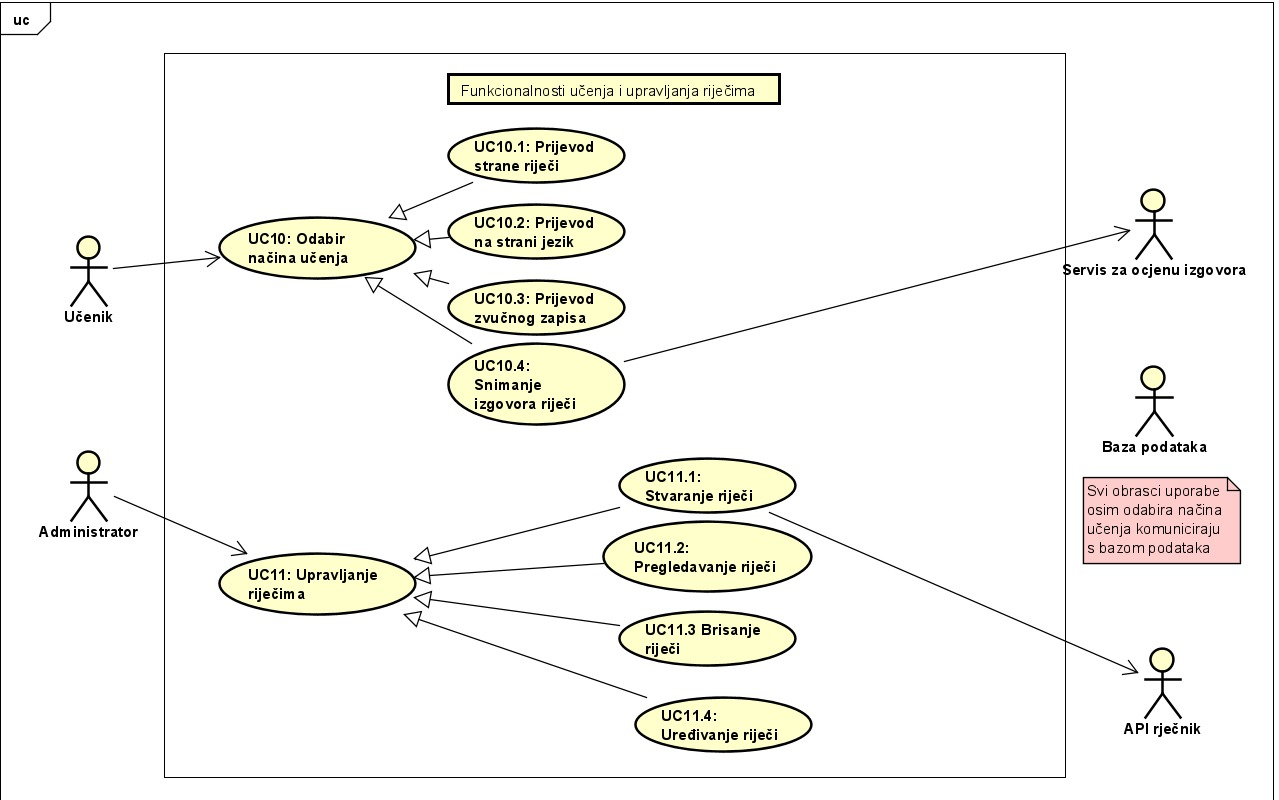
\includegraphics[scale=0.30]{dijagrami/dijagram1.jpg} 
						\centering
						\caption{Funkcionalnosti učenja i upravljanja riječima}
						\label{fig:dijagram1}
					\end{figure}
					
					\begin{figure}[H]
						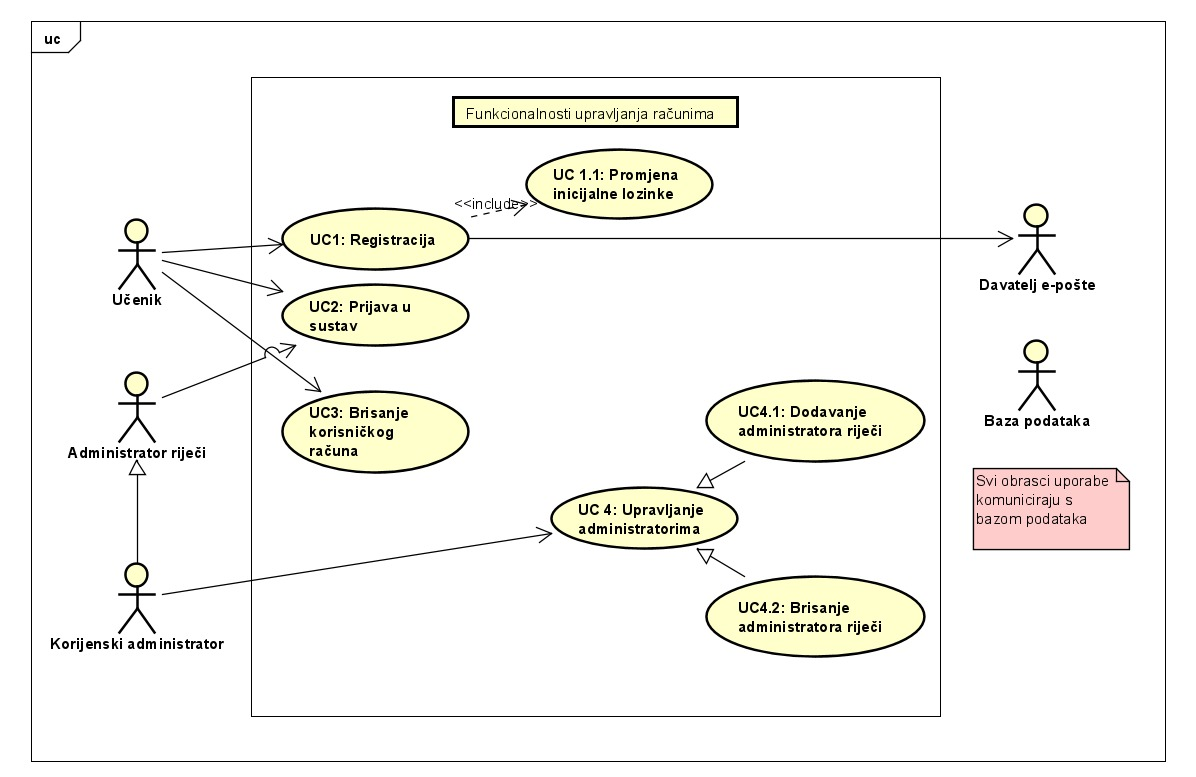
\includegraphics[scale=0.35]{dijagrami/dijagram2.jpg} 
						\centering
						\caption{Funkcionalnosti upravljanja računima}
						\label{fig:dijagram2}
					\end{figure}
					
					\begin{figure}[H]
						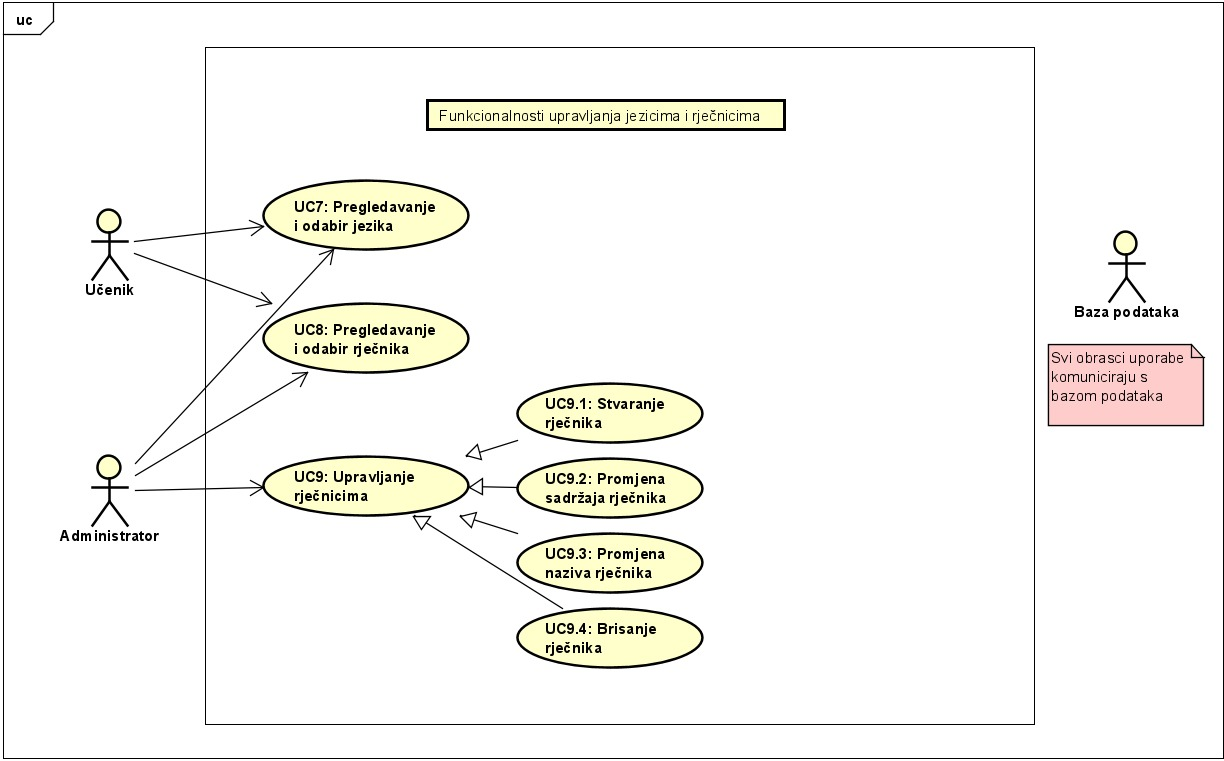
\includegraphics[scale=0.34]{dijagrami/dijagram3.jpg} 
						\centering
						\caption{Funkcionalnosti upravljanja jezicima i rječnicima}
						\label{fig:dijagram3}
					\end{figure}	
				
			\subsection{Sekvencijski dijagrami}
				
				\textbf{\textit{dio 1. revizije}}\\
				
				\textit{Nacrtati sekvencijske dijagrame koji modeliraju najvažnije dijelove sustava (max. 4 dijagrama). Ukoliko postoji nedoumica oko odabira, razjasniti s asistentom. Uz svaki dijagram napisati detaljni opis dijagrama.}
				\eject
	
				\section{Ostali zahtjevi}

				\begin{itemize}
					\item sustav korisniku daje povratnu informaciju o točnosti njegova odgovora
					\item sustav u razumnom vremenu prezentira riječi nakon odabira načina rada
					\item sustav mora imati potporu hrvatskih dijakritičkih znakova
					\item sustavu iz javne mreže pristupamo protokolom HTTPS
					\item sustav je dovoljno jednostavan i intuitivan za bilo koju dobnu skupinu korisnika 
					\item za korištenje sustava korisniku je potrebno poznavanje hrvatskog jezika
					\item rječnik mora imati barem 10 riječi
					\item prijevodi riječi moraju biti ispravni
				\end{itemize}
			 
			 
			 
	
	\chapter{Arhitektura i dizajn sustava}
		
Naš sustav se može podijeliti na pet glavnih podsustava koji međusobno komuniciraju:
\begin{description}
	\item[Web preglednik:] Lokalno instalirani program koji omogućuje prikaz sadržaja sa interneta. 
	Pomoću tog programa korisnik može poslati zahtjeve za 
	resursima ili poslati neke podatke web poslužitelju. Web preglednik, 
	nakon što dobije zatražene informacije od web poslužitelja, korisniku prikazuje ssadržaj.

	\item[Web poslužitelj:] Centralni podsustav aplikacije koji obrađuje višestruke zahtjeve korisnika. To 
	može biti zasebno računalo ili samo softver. Komunikaciju s klijentima ostvaruje preko
	HTTP protokola. Web poslužitelj može, na korisnički zahtjev, poslati datoteke ili primiti
	neke podatke koje može spremiti u bazu podataka.

	\item[Baza podataka:] Koristi se za pohranjivanje podataka web apliakcije. Sastavljena je od tablica koje
	predstavljaju entitete s određenim atributima koji su međusobno povezani definiranim
	odnosima. Web aplikacija često komunicira s bazom, povlačeći i davajući podatke bazi.

	\item[Servis za obradu izgovora:] Vanjski servis pomoću kojeg ocjenjujemo izgovor stranih riječi korisnika. Web
	aplikacija komunicira sa servisom preko aplikacijskog sučelja (API).

	\item[Servis za riječi:] Vanjski servis pomoću kojeg administratori lakše stvaraju rječi i, samim time,
	rječnike. Servispreko aplikacijskog sučelja (API) pruža značenja riječi i 
	popratne pomoćne fraze koje olakšavaju proces učenja.
\end{description}


\begin{figure}[h!]
	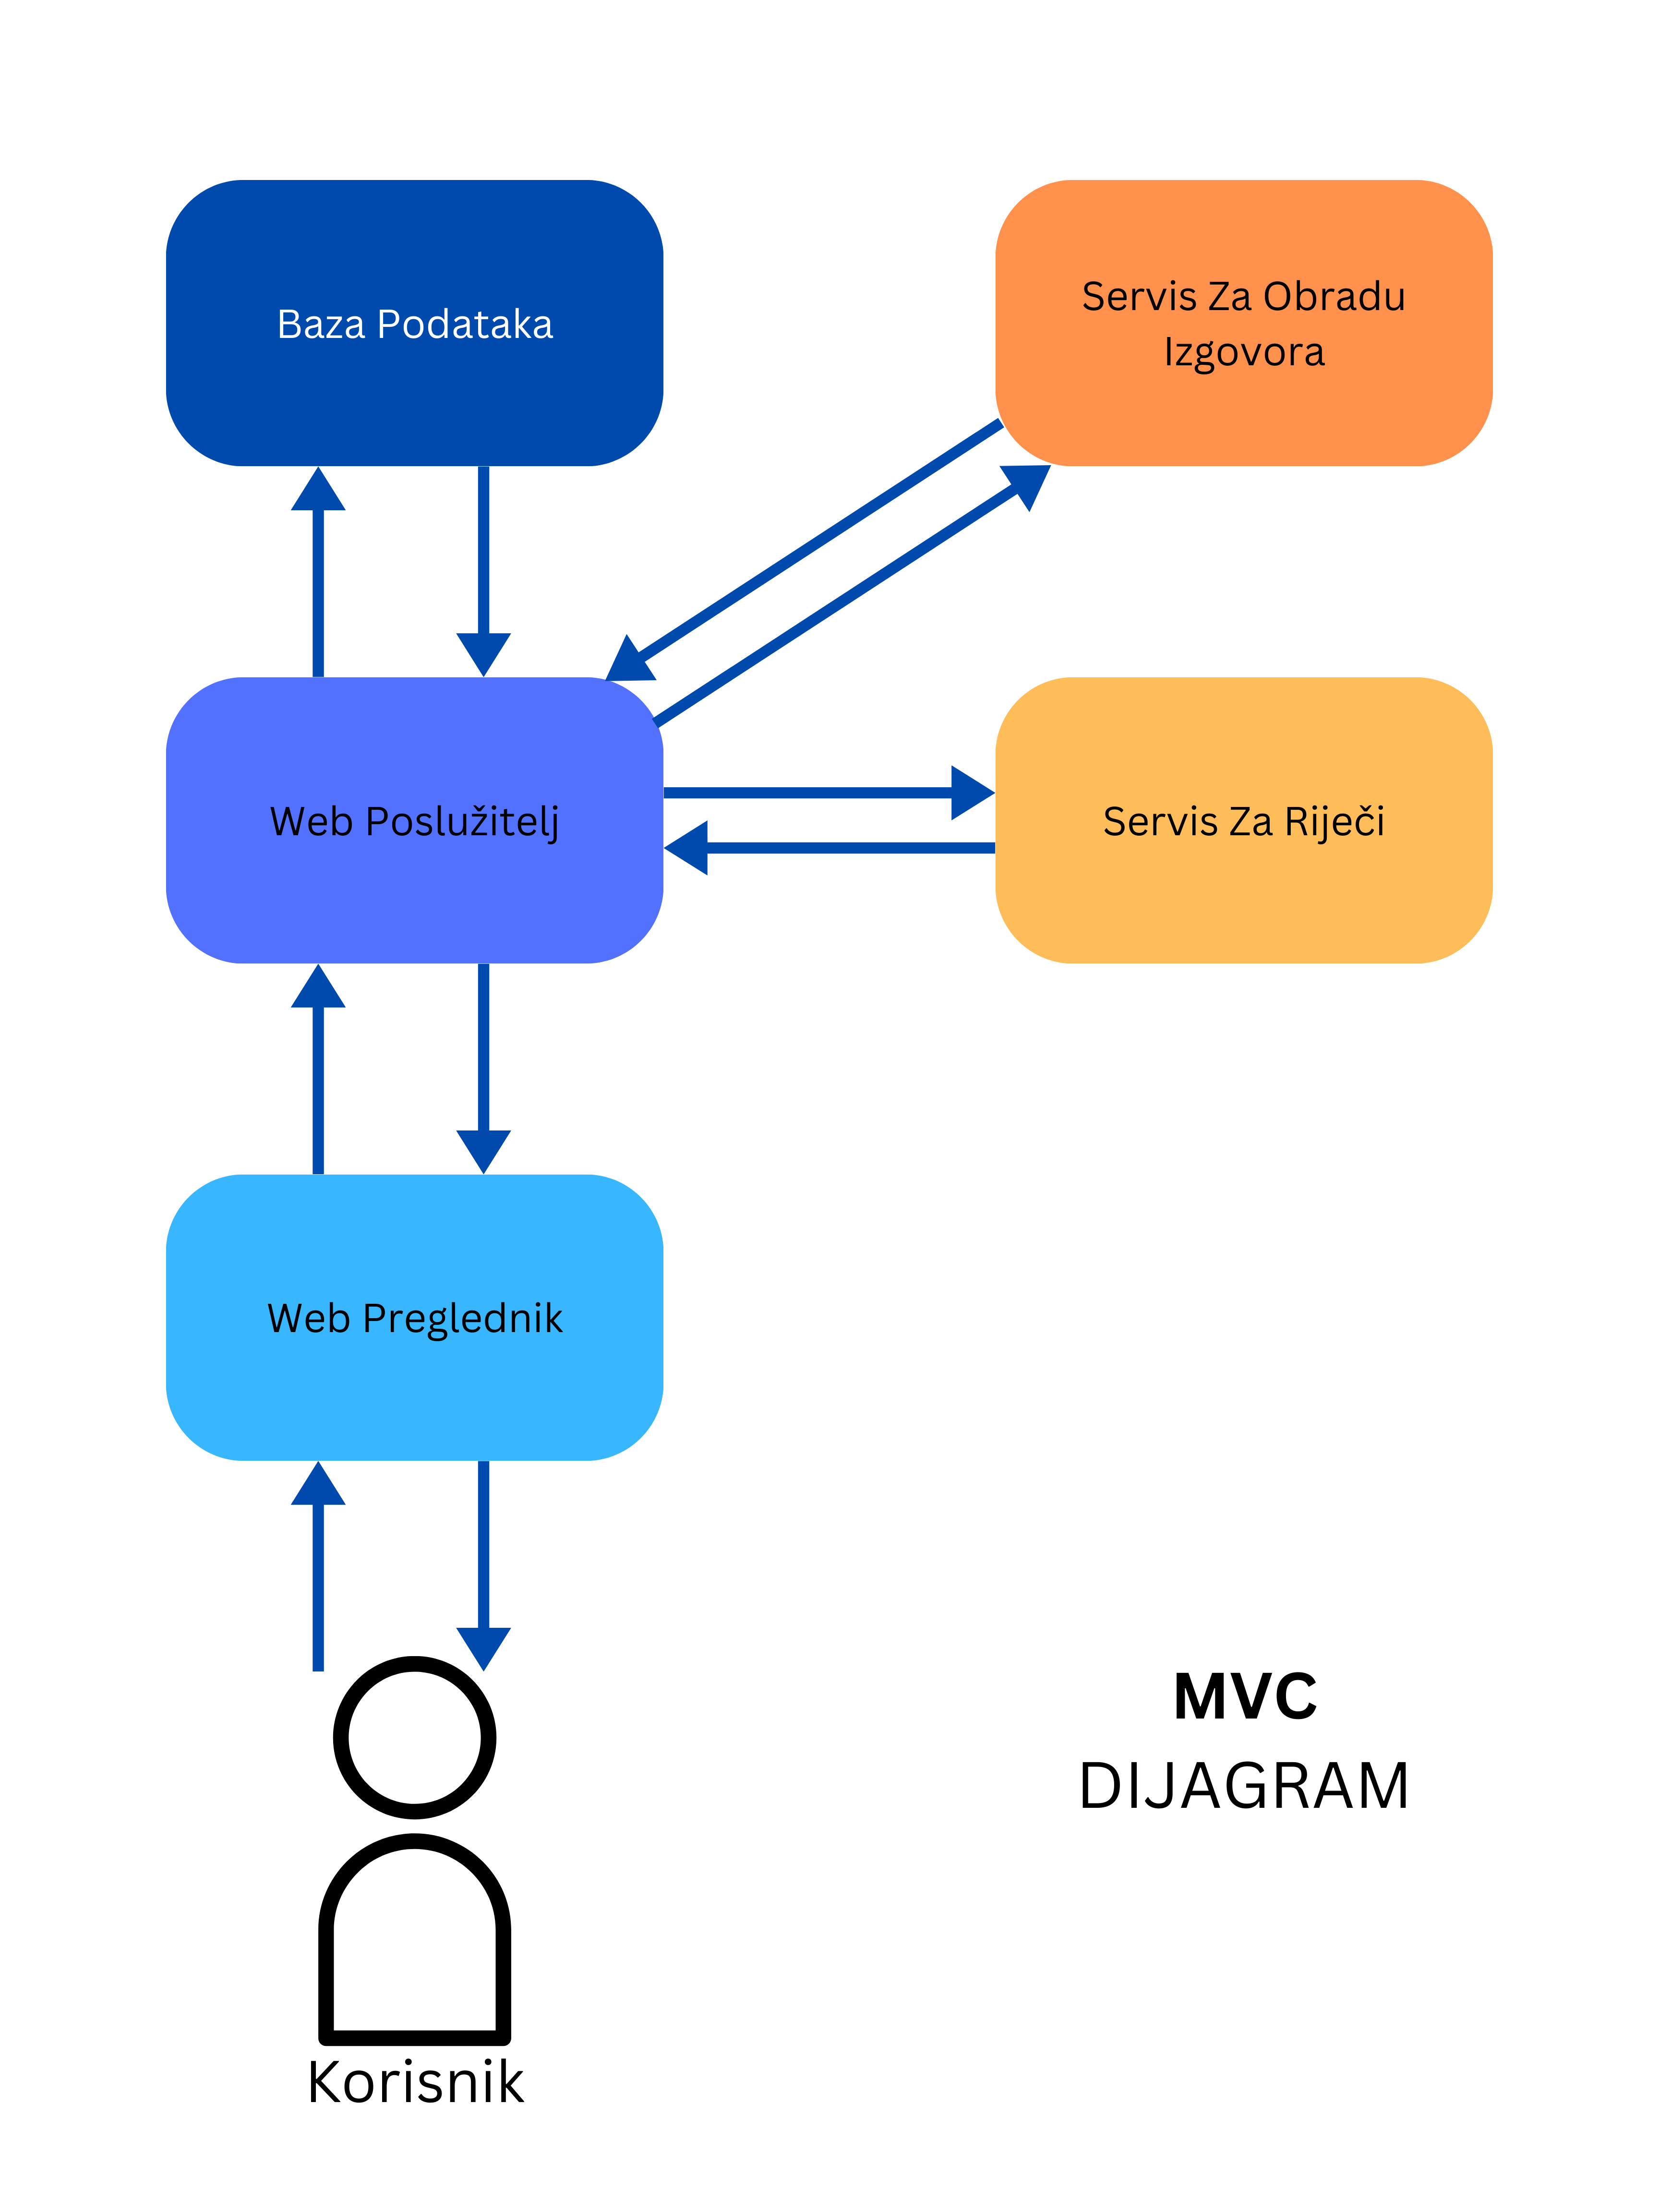
\includegraphics[scale=0.1]{dijagrami/Web Preglednik.png} 
	\centering
	\caption{Shema arhitekture aplikacije}
	\label{fig:mvc-arhitektura}
\end{figure}

\pagebreak

	U izradi aplikaciji koristili smo MVC obrazac dizajna softvera. Elementi tipičnog MVC koncepta su:

	\begin{description}
		\item[\textbf{Model}:] Struktura odgovorna za obradu i upravljanje podacima. 
		\item[\textbf{View}:] Sloj odgovoran za prikazivanje podataka korisnicima.
		\item[\textbf{Controller}:] Sloj koji upravlja logikom aplikacije te surađuje s modelom i pogledom.
	\end{description}


	Backend aplikacije izrađen je u Pythonu korištenjem Flask radnog okvira, dok je za bazu podataka korišten PostgreSQL. Frontend je izrađen u React-u. Također su za funkcionalnost apliakcije korišteni servisi za obradu izgovora i jezičnu provjeru. 
	
		

		

		\pagebreak		
		\section{Baza podataka}

		Naš sustav koristi bazu podataka koja se temelji na relacijskom modelu podataka i koristi tablice (relacije) za organizaciju i pohranu podataka. Entiteti naše baze su: 
		\begin{itemize}
			\item Jezik
			\item Rječnik
			\item Riječ
			\item Korisnik
			\item Fraza
			\item Posuda
		\end{itemize}

			
			
		
			\subsection{Opis tablica}
			

				\textit{Svaku tablicu je potrebno opisati po zadanom predlošku. Lijevo se nalazi točno ime varijable u bazi podataka, u sredini se nalazi tip podataka, a desno se nalazi opis varijable. Svjetlozelenom bojom označite primarni ključ. Svjetlo plavom označite strani ključ}
				
				
				\begin{longtblr}[
					label=none,
					entry=none
					]{
						width = \textwidth,
						colspec={|X[6,l]|X[6, l]|X[20, l]|}, 
						rowhead = 1,
					} %definicija širine tablice, širine stupaca, poravnanje i broja redaka naslova tablice
					\hline \SetCell[c=3]{c}{\textbf{korisnik - ime tablice}}	 \\ \hline[3pt]
					\SetCell{LightGreen}IDKorisnik & INT	&  	Lorem ipsum dolor sit amet, consectetur adipiscing elit, sed do eiusmod  	\\ \hline
					korisnickoIme	& VARCHAR &   	\\ \hline 
					email & VARCHAR &   \\ \hline 
					ime & VARCHAR	&  		\\ \hline 
					\SetCell{LightBlue} primjer	& VARCHAR &   	\\ \hline 
				\end{longtblr}
				
				
			
			\subsection{Dijagram baze podataka}
				\textit{ U ovom potpoglavlju potrebno je umetnuti dijagram baze podataka. Primarni i strani ključevi moraju biti označeni, a tablice povezane. Bazu podataka je potrebno normalizirati. Podsjetite se kolegija "Baze podataka".}

				\begin{figure}[H]
					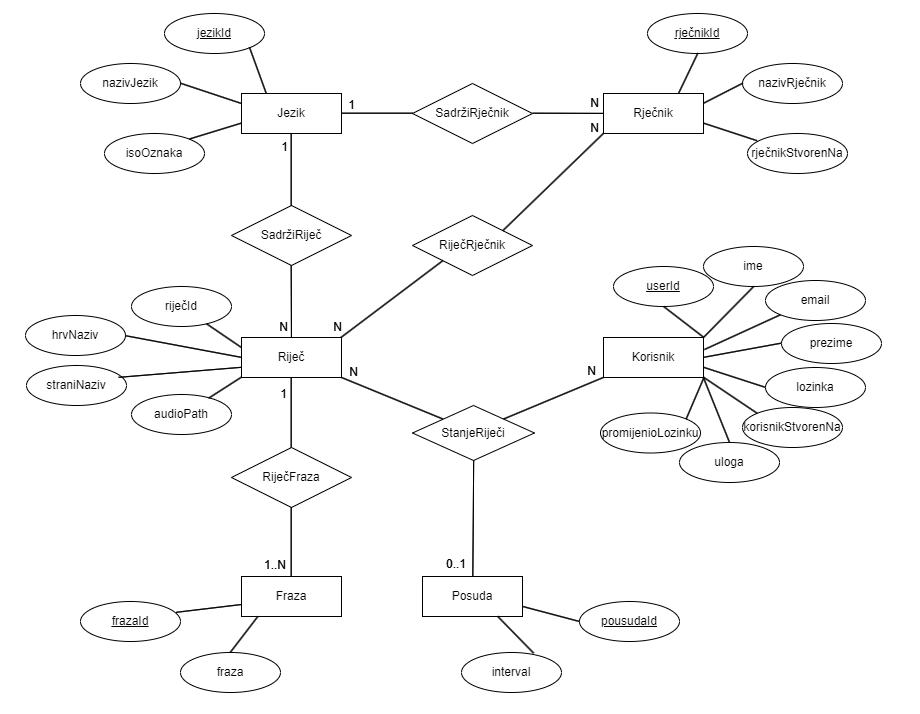
\includegraphics[scale=0.5]{dijagrami/ER_model_BP_3.png}
					\centering
					\caption{ER model baze podataka}
					\label{fig:dijagram_ER-BP}
				\end{figure}
			
			\eject
			
			
		\section{Dijagram razreda}
		
			\textit{Potrebno je priložiti dijagram razreda s pripadajućim opisom. Zbog preglednosti je moguće dijagram razlomiti na više njih, ali moraju biti grupirani prema sličnim razinama apstrakcije i srodnim funkcionalnostima.}\\
			
			\textbf{\textit{dio 1. revizije}}\\
			
			\textit{Prilikom prve predaje projekta, potrebno je priložiti potpuno razrađen dijagram razreda vezan uz \textbf{generičku funkcionalnost} sustava. Ostale funkcionalnosti trebaju biti idejno razrađene u dijagramu sa sljedećim komponentama: nazivi razreda, nazivi metoda i vrste pristupa metodama (npr. javni, zaštićeni), nazivi atributa razreda, veze i odnosi između razreda.}\\
			
			\textbf{\textit{dio 2. revizije}}\\			
			
			\textit{Prilikom druge predaje projekta dijagram razreda i opisi moraju odgovarati stvarnom stanju implementacije}
			
			
			
			\eject
		
		\section{Dijagram stanja}
			
			
			\textbf{\textit{dio 2. revizije}}\\
			
			\textit{Potrebno je priložiti dijagram stanja i opisati ga. Dovoljan je jedan dijagram stanja koji prikazuje \textbf{značajan dio funkcionalnosti} sustava. Na primjer, stanja korisničkog sučelja i tijek korištenja neke ključne funkcionalnosti jesu značajan dio sustava, a registracija i prijava nisu. }
			
			
			\eject 
		
		\section{Dijagram aktivnosti}
			
			\textbf{\textit{dio 2. revizije}}\\
			
			 \textit{Potrebno je priložiti dijagram aktivnosti s pripadajućim opisom. Dijagram aktivnosti treba prikazivati značajan dio sustava.}
			
			\eject
		\section{Dijagram komponenti}
		
			\textbf{\textit{dio 2. revizije}}\\
		
			 \textit{Potrebno je priložiti dijagram komponenti s pripadajućim opisom. Dijagram komponenti treba prikazivati strukturu cijele aplikacije.}
	\chapter{Implementacija i korisničko sučelje}
		
		
		\section{Korištene tehnologije i alati}
		
			\textbf{\textit{dio 2. revizije}}
			
			 \textit{Detaljno navesti sve tehnologije i alate koji su primijenjeni pri izradi dokumentacije i aplikacije. Ukratko ih opisati, te navesti njihovo značenje i mjesto primjene. Za svaki navedeni alat i tehnologiju je potrebno \textbf{navesti internet poveznicu} gdje se mogu preuzeti ili više saznati o njima}.
			
			
			\eject 
		
	
		\section{Ispitivanje programskog rješenja}
			
			\textbf{\textit{dio 2. revizije}}\\
			
			 \textit{U ovom poglavlju je potrebno opisati provedbu ispitivanja implementiranih funkcionalnosti na razini komponenti i na razini cijelog sustava s prikazom odabranih ispitnih slučajeva. Studenti trebaju ispitati temeljnu funkcionalnost i rubne uvjete.}
	
			
			\subsection{Ispitivanje komponenti}
			\textit{Potrebno je provesti ispitivanje jedinica (engl. unit testing) nad razredima koji implementiraju temeljne funkcionalnosti. Razraditi \textbf{minimalno 6 ispitnih slučajeva} u kojima će se ispitati redovni slučajevi, rubni uvjeti te izazivanje pogreške (engl. exception throwing). Poželjno je stvoriti i ispitni slučaj koji koristi funkcionalnosti koje nisu implementirane. Potrebno je priložiti izvorni kôd svih ispitnih slučajeva te prikaz rezultata izvođenja ispita u razvojnom okruženju (prolaz/pad ispita). }
			
			 

			\subsection{Ispitivanje sustava}
Ispitivanje sustava ostvareno je Selenium WebDriverom u Pythonu. Provedeni testovi s kodom priloženi su u nastavku.
\break
Prvi ispitni slučaj obrađuje pokušaj prijave emailom koji ne postoji u sustavu. Očekivani izlaz je neuspjeh prijave.

\lstset{language=Python, xleftmargin=0pt}
\begin{lstlisting}
def test1() -> bool:
    url = "http://localhost:3000/login"
    driver.get(url)
    driver.find_element(By.ID, "email").send_keys("osoba@osoba.com")
    driver.find_element(By.ID, "password").send_keys("123456")
    driver.find_element(By.CSS_SELECTOR, "button[type='submit']").click()

    if driver.current_url.endswith("/login"):
        return True
    else:
        return False
\end{lstlisting}

Drugi ispitni slučaj obrađuje pokušaj registracije s emailom u neispravnom formatu. Očekivani izlaz je neuspjeh registracije.

\lstset{language=Python, xleftmargin=0pt}
\begin{lstlisting}
def test2() -> bool:
    url = "http://localhost:3000/login"
    driver.get(url)
    driver.find_element(By.CSS_SELECTOR, "button[type='button']").click()
    driver.find_element(By.ID, "firstname").send_keys("Osoba")
    driver.find_element(By.ID, "lastname").send_keys("Osoba")
    driver.find_element(By.ID, "email").send_keys("osoba.com")
    driver.find_element(By.CSS_SELECTOR, "button[type='submit']").click()

    if driver.current_url.endswith("/register"):
        return True
    else:
        return False
\end{lstlisting}

Treći ispitni slučaj obrađuje pokušaj registracije s svim valjanim podacima. Očekivani izlaz je uspješna registracija i preusmjeravanje.

\lstset{language=Python, xleftmargin=0pt}
\begin{lstlisting}
def test3() -> bool:
    url = "http://localhost:3000/login"
    driver.get(url)
    driver.find_element(By.CSS_SELECTOR, "button[type='button']").click()
    driver.find_element(By.ID, "firstname").send_keys("Osoba")
    driver.find_element(By.ID, "lastname").send_keys("Osoba")
    driver.find_element(By.ID, "email").send_keys("osoba@osoba.com")
    driver.find_element(By.CSS_SELECTOR, "button[type='submit']").click()

    if driver.current_url.endswith("/register"):
        return False
    else:
        return True
\end{lstlisting}

Četvrti ispitni slučaj obrađuje pokušaj prijave s postojećim emailom, ali s neispravnom lozinkom. Očekivani izlaz je neuspjeh prijave.

\lstset{language=Python, xleftmargin=0pt}
\begin{lstlisting}
def test4() -> bool:
    url = "http://localhost:3000/login"
    driver.get(url)
    driver.find_element(By.ID, "email").send_keys("admin@admin.com")
    driver.find_element(By.ID, "password").send_keys("123456")
    driver.find_element(By.CSS_SELECTOR, "button[type='submit']").click()

    if driver.current_url.endswith("/login"):
        return True
    else:
        return False
\end{lstlisting}

Peti ispitni slučaj obrađuje pokušaj prijave s ispravnim emailom i lozinkom. Očekivani izlaz je uspješna prijava i preusmjeravanje. 

\lstset{language=Python, xleftmargin=0pt}
\begin{lstlisting}
def test5() -> bool:
    url = "http://localhost:3000/login"
    driver.get(url)
    driver.find_element(By.ID, "email").send_keys("admin@admin.com")
    driver.find_element(By.ID, "password").send_keys("progi123")
    driver.find_element(By.CSS_SELECTOR, "button[type='submit']").click()
    time.sleep(0.5)

    if driver.current_url.endswith("/login"):
        return False
    else:
        return True
\end{lstlisting}

Na slici 5.1 prikazan je screenshot terminala nakon pokretanja navedenih pet ispitnih slučajeva.

\begin{figure}[htp]
    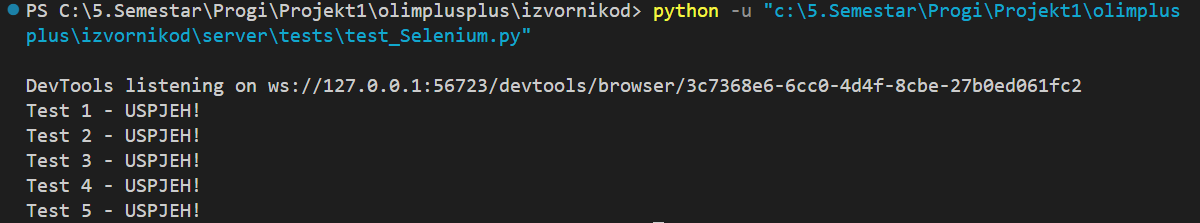
\includegraphics[scale=0.5]{dijagrami/testsScreenshot.png}
    \centering
    \caption{Rezultati ispitivanja Selenium WebDriverom}
\end{figure}

\eject

		
		\section{Dijagram razmještaja}
			
		\begin{figure}[htp]
			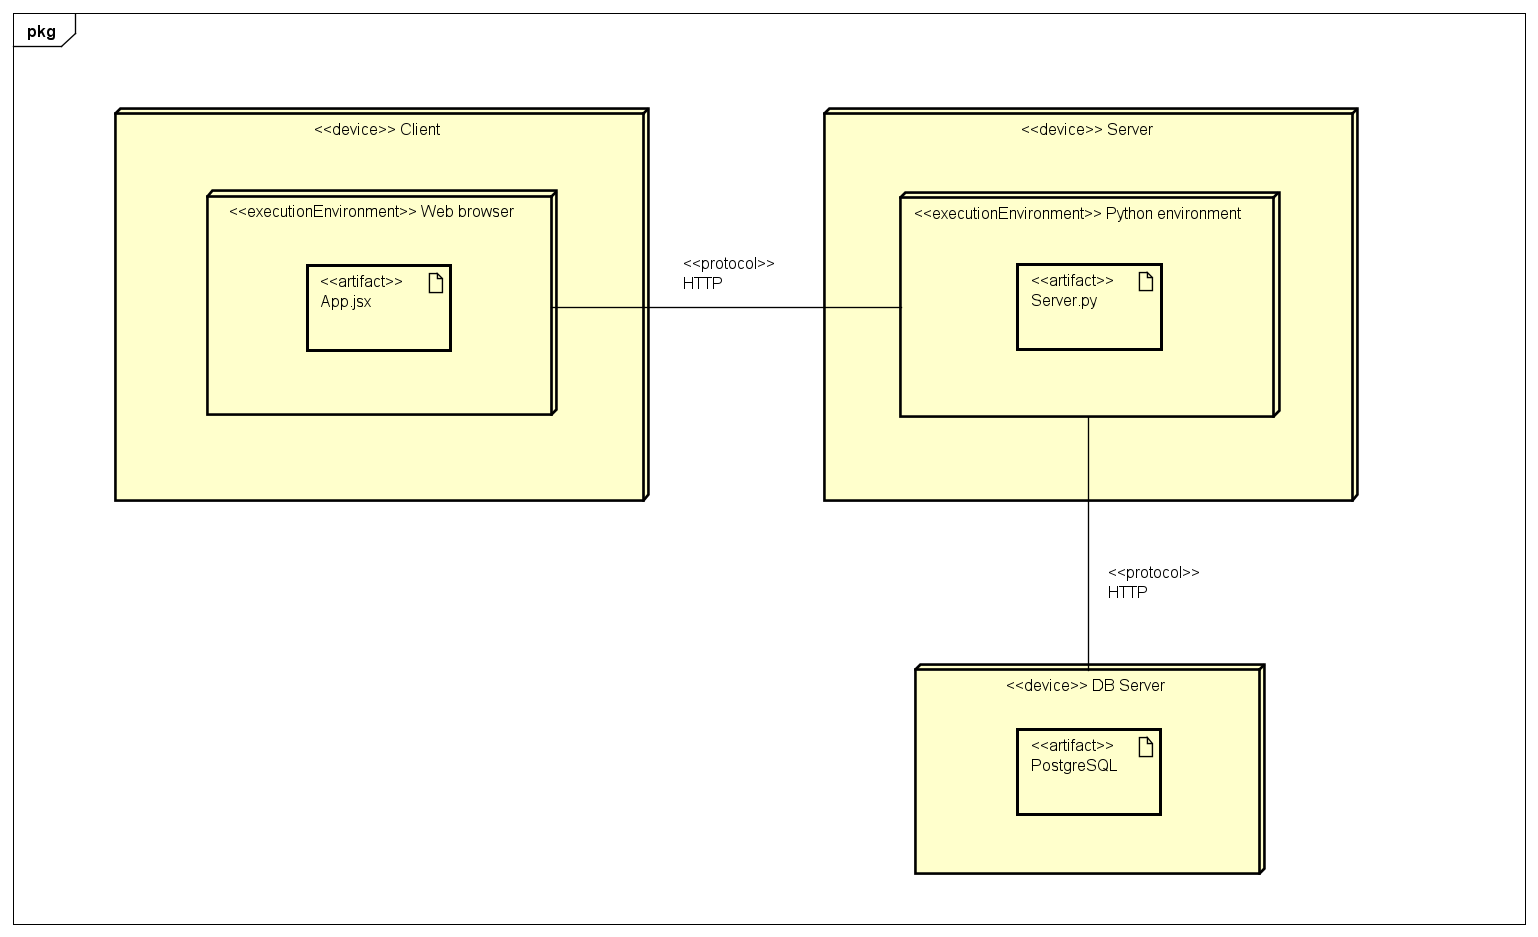
\includegraphics[scale=0.4]{dijagrami/DeploymentDiagram0.png}
			\centering
			\caption{Dijagram razmještaja}
		\end{figure}
		
		\section{Upute za puštanje u pogon}
		
			\textbf{\textit{dio 2. revizije}}\\
		
			 \textit{U ovom poglavlju potrebno je dati upute za puštanje u pogon (engl. deployment) ostvarene aplikacije. Na primjer, za web aplikacije, opisati postupak kojim se od izvornog kôda dolazi do potpuno postavljene baze podataka i poslužitelja koji odgovara na upite korisnika. Za mobilnu aplikaciju, postupak kojim se aplikacija izgradi, te postavi na neku od trgovina. Za stolnu (engl. desktop) aplikaciju, postupak kojim se aplikacija instalira na računalo. Ukoliko mobilne i stolne aplikacije komuniciraju s poslužiteljem i/ili bazom podataka, opisati i postupak njihovog postavljanja. Pri izradi uputa preporučuje se \textbf{naglasiti korake instalacije uporabom natuknica} te koristiti što je više moguće \textbf{slike ekrana} (engl. screenshots) kako bi upute bile jasne i jednostavne za slijediti.}
			
			
			 \textit{Dovršenu aplikaciju potrebno je pokrenuti na javno dostupnom poslužitelju. Studentima se preporuča korištenje neke od sljedećih besplatnih usluga: \href{https://aws.amazon.com/}{Amazon AWS}, \href{https://azure.microsoft.com/en-us/}{Microsoft Azure} ili \href{https://www.heroku.com/}{Heroku}. Mobilne aplikacije trebaju biti objavljene na F-Droid, Google Play ili Amazon App trgovini.}
			
			
			\eject 
	\chapter{Zaključak i budući rad}

\par Razvoj projekta je bilo važno iskustvo za sve članove tima. Dobili smo uvid u alate za komunikaciju
ideja, kao što su stečene i vještine sinkronizacije sa drugim članovima. Naučeno je puno o konkretnom razvoju
aplikacija na webu, kao i o Reactu. Vrijeme razvoja je bilo definirano količinama znanja individualnih članova tima, 
te da ponovno pravimo isti projekt sa svime naučenim, išlo bi brže.
\par Puno vremena je bilo uloženo u idejnu razradu aplikacije, te smo se posvetili detaljima funkcionalnih
zahtjeva i razrade svih obrazaca uporabe prije nego što smo krenuli programirati, što je u konačnici uštedilo
puno vremena. Nismo imali dvoumljenja oko implementacije, samo smo mogli pisati po već razrađenim
obrascima. 
\par Za bržu i kvalitetniju izradu projekta bi samo bilo potrebno da svi članovi imaju istu količinu
znanja vezanu za odabrani radni okvir, kao i sličnu količinu iskustva u izradi web aplikacija. Puno stvari
u razvoju na webu se ponavlja, projekti imaju slične strukture datoteka, koriste se isti programski obrasci
kao rješenje dobro poznatih problema. Izrada baze podataka je donekle standardiziran postupak, 
povezivanje na istu i povlačenje podataka se može napraviti na više načina. Sve se svodi na odabir nekih od 
svih dostupnih tehnologija, te iskustvo s radom u istim. Korisničko sučelje se može napraviti relativno brzo
uz pomoć biblioteka i radnih okvira. Puno gotovih rješenja za web već postoji, vještina ih je znati spojiti
i znati kako te bibilioteke međusobno komuniciraju. 
\par Glede perspektiva za nastavak rada u projektnoj grupi, bilo kakav budući rad može biti samo lakši,
budući da je tim prošao kroz svoje ranije faze, te svi članovi lakše znaju komunicirati jedni s drugima i 
uskočiti tamo gdje treba. Svi su upoznati s vlastitim snagama i slabostima.
\par Sve tražene funkcionalnsoti projektnog zadatka su implementirane i razrađene. 


\eject
	\chapter*{Popis literature}
		\addcontentsline{toc}{chapter}{Popis literature}
	 	
 		\textbf{\textit{Kontinuirano osvježavanje}}
	
		\textit{Popisati sve reference i literaturu koja je pomogla pri ostvarivanju projekta.}
		
		
		\begin{enumerate}
			
			
			\item  Programsko inženjerstvo, FER ZEMRIS, \url{http://www.fer.hr/predmet/proinz}
			
			\item  I. Sommerville, "Software engineering", 8th ed, Addison Wesley, 2007.
			
			\item  T.C.Lethbridge, R.Langaniere, "Object-Oriented Software Engineering", 2nd ed. McGraw-Hill, 2005.
			
			\item  I. Marsic, "Software engineering book", Department of Electrical and Computer Engineering, Rutgers University, \url{http://www.ece.rutgers.edu/~marsic/books/SE}
			
			\item  The Unified Modeling Language, \url{https://www.uml-diagrams.org/}
			
			\item  Astah Community, \url{http://astah.net/editions/uml-new}
		\end{enumerate}
		
		 
	
	
	\begingroup
	\renewcommand*\listfigurename{Indeks slika i dijagrama}
	%\renewcommand*\listtablename{Indeks tablica}
	%\let\clearpage\relax
	\listoffigures
	%\vspace{10mm}
	%\listoftables
	\endgroup
	\addcontentsline{toc}{chapter}{Indeks slika i dijagrama}


	
	\eject 
		
	\chapter*{Dodatak: Prikaz aktivnosti grupe}
		\addcontentsline{toc}{chapter}{Dodatak: Prikaz aktivnosti grupe}
		
		\section*{Dnevnik sastajanja}
		
		\textbf{\textit{Kontinuirano osvježavanje}}\\
		
		 \textit{U ovom dijelu potrebno je redovito osvježavati dnevnik sastajanja prema predlošku.}
		
		\begin{packed_enum}
			\item  sastanak
			
			\item[] \begin{packed_item}
				\item Datum: u ovom formatu: \today
				\item Prisustvovali: I.Prezime, I.Prezime
				\item Teme sastanka:
				\begin{packed_item}
					\item  opis prve teme
					\item  opis druge teme
				\end{packed_item}
			\end{packed_item}
			
			\item  sastanak
			\item[] \begin{packed_item}
				\item Datum: u ovom formatu: \today
				\item Prisustvovali: I.Prezime, I.Prezime
				\item Teme sastanka:
				\begin{packed_item}
					\item  opis prve teme
					\item  opis druge teme
				\end{packed_item}
			\end{packed_item}
			
			%
			
		\end{packed_enum}
		
		\eject
		\section*{Tablica aktivnosti}
		
			\textbf{\textit{Kontinuirano osvježavanje}}\\
			
			 \textit{Napomena: Doprinose u aktivnostima treba navesti u satima po članovima grupe po aktivnosti.}

			\begin{longtblr}[
					label=none,
				]{
					vlines,hlines,
					width = \textwidth,
					colspec={X[7, l]X[1, c]X[1, c]X[1, c]X[1, c]X[1, c]X[1, c]X[1, c]}, 
					vline{1} = {1}{text=\clap{}},
					hline{1} = {1}{text=\clap{}},
					rowhead = 1,
				} 
			
				\SetCell[c=1]{c}{} & \SetCell[c=1]{c}{\rotatebox{90}{\textbf{Duje Štolfa}}} & 
				\SetCell[c=1]{c}{\rotatebox{90}{\textbf{Karlo Kuzle}}} &
				\SetCell[c=1]{c}{\rotatebox{90}{\textbf{Ivo Žilić}}} & 
				\SetCell[c=1]{c}{\rotatebox{90}{\textbf{Frane Kuzmanić }}} &
				\SetCell[c=1]{c}{\rotatebox{90}{\textbf{Ime Prezime }}} & 
				\SetCell[c=1]{c}{\rotatebox{90}{\textbf{Gabrijel Čobanov}}} &
				\SetCell[c=1]{c}{\rotatebox{90}{\textbf{Nikša Brala}}} \\  
				Upravljanje projektom 		&  &  &  &  &  &  & \\ 
				Opis projektnog zadatka 	&  &  &  &  &  &  & \\ 
				
				Funkcionalni zahtjevi       &  &  &  &  &  &  &  \\ 
				Opis pojedinih obrazaca 	&  &  &  &  &  &  &  \\ 
				Dijagram obrazaca 			&  &  &  &  &  &  &  \\ 
				Sekvencijski dijagrami 		&  &  &  &  &  &  &  \\ 
				Opis ostalih zahtjeva 		&  &  &  &  &  &  &  \\ 

				Arhitektura i dizajn sustava	 &  &  &  &  &  &  &  \\ 
				Baza podataka				&  &  &  &  &  &  &   \\ 
				Dijagram razreda 			&  &  &  &  &  &  &   \\ 
				Dijagram stanja				&  &  &  &  &  &  &  \\ 
				Dijagram aktivnosti 		&  &  &  &  &  &  &  \\ 
				Dijagram komponenti			&  &  &  &  &  &  &  \\ 
				Korištene tehnologije i alati 		&  &  &  &  &  &  &  \\ 
				Ispitivanje programskog rješenja 	&  &  &  &  &  &  &  \\ 
				Dijagram razmještaja			&  &  &  &  &  &  &  \\ 
				Upute za puštanje u pogon 		&  &  &  &  &  &  &  \\  
				Dnevnik sastajanja 			&  &  &  &  &  &  &  \\ 
				Zaključak i budući rad 		&  &  &  &  &  &  &  \\  
				Popis literature 			&  &  &  &  &  &  &  \\  
				&  &  &  &  &  &  &  \\ \hline 
				\textit{Dodatne stavke kako ste podijelili izradu aplikacije} 			&  &  &  &  &  &  &  \\ 
				\textit{npr. izrada početne stranice} 				&  &  &  &  &  &  &  \\  
				\textit{izrada baze podataka} 		 			&  &  &  &  &  &  & \\  
				\textit{spajanje s bazom podataka} 							&  &  &  &  &  &  &  \\ 
				\textit{back end} 							&  &  &  &  &  &  &  \\  
				 							&  &  &  &  &  &  &\\ 
			\end{longtblr}
					
					
		\eject
		\section*{Dijagrami pregleda promjena}
		
		\textbf{\textit{dio 2. revizije}}\\
		
		\textit{Prenijeti dijagram pregleda promjena nad datotekama projekta. Potrebno je na kraju projekta generirane grafove s gitlaba prenijeti u ovo poglavlje dokumentacije. Dijagrami za vlastiti projekt se mogu preuzeti s gitlab.com stranice, u izborniku Repository, pritiskom na stavku Contributors.}
		
	


\end{document} %naredbe i tekst nakon ove naredbe ne ulaze u izgrađen dokument 


